\documentclass[main.tex]{subfiles}

\begin{document}
\section{Характеристики}
\subsection{Избор}
За стойности на характеристичните вектори ще използваме енергията на всяка една от вълните за всеки електрод. Използването само на разликите в енергиите между двете половини на мозъка, както се предлага в много статии, не доведе до по-добър резултат. Сега нека видим как се извличат енергиите.

\subsection{Извличане}

\begin{minipage}{0.45\textwidth}
        \begin{figure}[H]
                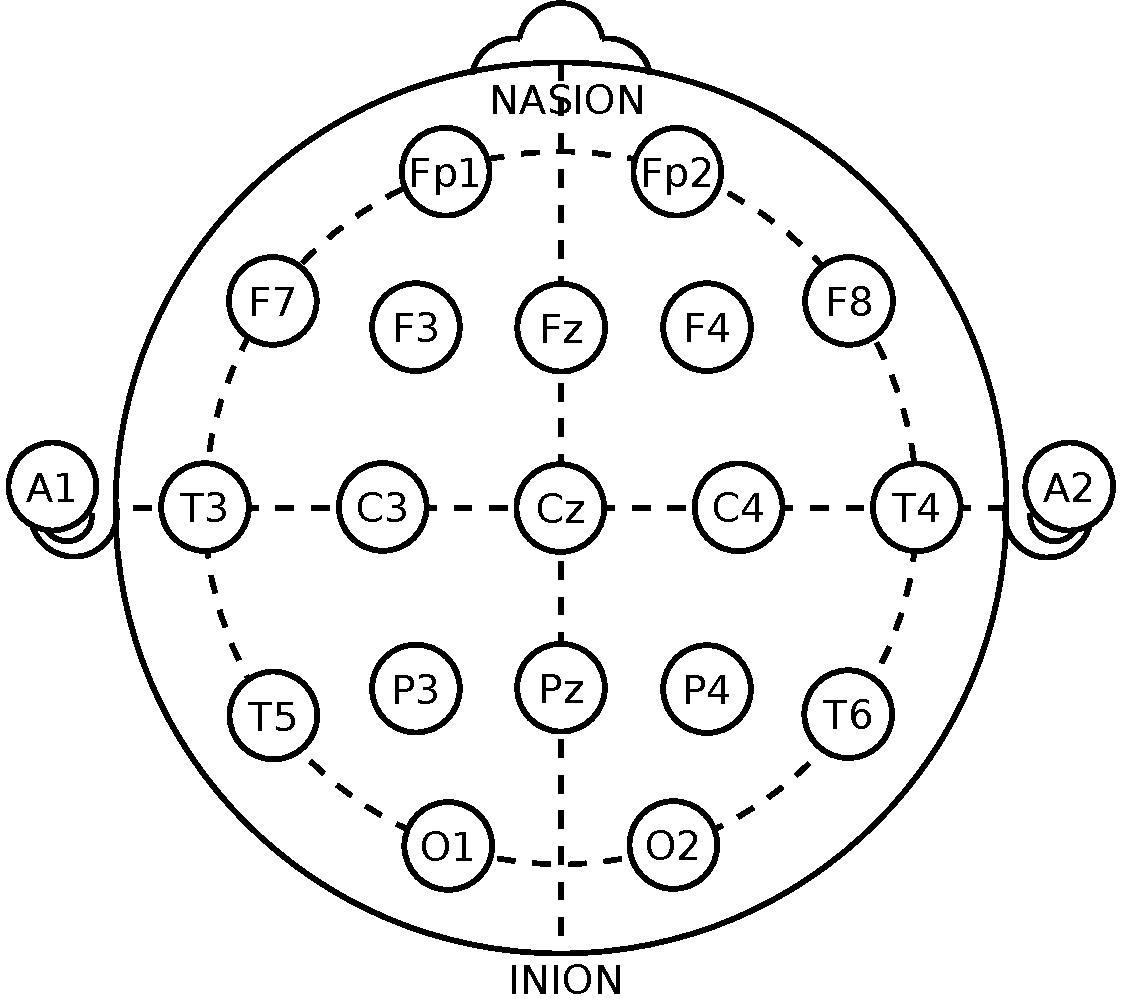
\includegraphics[width=\textwidth]{10_20}
                \caption{Система за разпределяне на електроди 10-20}
                \label{fig:brain_char:1}
        \end{figure}
\end{minipage} \hfill
\begin{minipage}{0.45\textwidth}
        Електродите се нагласят по стандартната схема 10-20. Разпределението им е показано на \autoref{fig:brain_char:1}. Електроди $A1$ и $A2$ се наричат референтни. Те не са разположени по скалпа и целта им е да филтрират шума, като накрая осреднената им стойност се изважда от стойностите на останалите електроди автоматично. Електроенцефалографът записва информация за всеки от 19-те електрода с честота 500Hz, тоест за всяка секунда получаваме 500 деветнадесет-мерни вектора.
\end{minipage}
Данните от енцефалографа се прочитат, като обработката на сигнала от всеки електрод е следната:
\begin{enumerate}
        \item Целият сигнал за даден електрод се прочита
        \item Сигналът се разбива на фреймове с дължина $200ms$ и стъпка $150ms$. На всеки фрейм се прави Хеминг прозорец и се намира Фурие преобразуванието
        \item Енергията на Фурие коефициентите се сумира в съответните честотните ленти, отговарящи на дадена вълна. Тъй като се асоциират със състояние на дълбок сън, $\theta$ вълните не се взимат предвид. В такъв случай имаме четири честотни ленти: 4-8Hz($\delta$), 8-12Hz($\alpha$), 12-30Hz($\beta$), 30-50Hz($\gamma$)
\end{enumerate}
В крайна сметка за всеки от подадените файлове, съответстващи на електроенцефалограма, получаваме за всеки електрод натрупаните стойности в четирите честотни ленти за всеки фрейм. Ако броят на фреймовете е $F$, то имаме $F$ на брой $(19\times4)$ мерни вектора.
\end{document}
